% Это основная команда, с которой начинается любой \LaTeX-файл. Она отвечает за тип документа, с которым связаны основные правил оформления текста.
\documentclass{article}[a4paper, 14pt]

% Здесь идет преамбула документа, тут пишутся команды, которые настраивают LaTeX окружение, подключаете внешние пакеты, определяете свои команды и окружения. В данном случае я это делаю в отдельных файлах, а тут подключаю эти файлы.

% Здесь я подключаю разные стилевые пакеты. Например возможности набирать особые символы или возможность компилировать русский текст. Подробное описание внутри.
\usepackage{packages}

% Здесь я определяю разные окружения, например, теоремы, определения, замечания и так далее. У этих окружений разные стили оформления, кроме того, эти окружения могут быть нумерованными или нет. Все подробно объяснено внутри.
\usepackage{environments}

% Здесь я определяю разные команды, которых нет в LaTeX, но мне нужны, например, команда \tr для обозначения следа матрицы. Или я переопределяю LaTeX команды, которые работают не так, как мне хотелось бы. Типичный пример мнимая и вещественная часть комплексного числа \Im, \Re. В оригинале они выглядят не так, как мы привыкли. Кроме того, \Im еще используется и для обозначения образа линейного отображения. Подробнее описано внутри.
\usepackage{commands}

% Пакет для титульника проекта
\usepackage{titlepage}

% Пакеты для отображения картинок
\usepackage{graphicx}
\usepackage{float}
\usepackage{wrapfig}

%
%\usepackage[unicode=true, colorlinks=true, linkcolor=blue, urlcolor=blue]{hyperref}


% Здесь задаем параметры титульной страницы
\setUDK{192.168.1.1}
% Выбрать одно из двух
%\setToResearch
%\setToProgram
\setToPractice

\setTitle{Мобильное приложение для отслеживания привычек}


\setStageOne

%сюда можно воткнуть картинку подписи
\setStudentSgn{}

\providecommand{\studentCompleted}{Выполнил студент}
\providecommand{\student}{TestStudent}
\providecommand{\group}{404}

\setStudent{\student}
\setGroup{\group}

\setStudentDate{20.10.2022}
\setAdvisor{Колесниченко Елена Юрьевна}
\setAdvisorTitle{департамент больших данных и информационного поиска ФКН ВШЭ, доцент}
\setAdvisorAffiliation{ООО <<Яндекс. Технологии>>}
\setAdvisorDate{24.10.2022}
\setGrade{--}
%сюда можно воткнуть картинку подписи
\setAdvisorSgn{}
\setYear{2022}

\setStudentCompleted{\studentCompleted}

\linespread{1.2}
\urlstyle{same}

\bibliographystyle{Bibliography/gost-numeric.bbx}
\usepackage[parentracker=true,
backend=biber,
hyperref=true,
bibencoding=utf8,
language=auto,
autolang=other,
citestyle=gost-numeric,
defernumbers=true,
bibstyle=gost-numeric,
sorting=ntvy,
maxbibnames=99,
]{biblatex}

\addbibresource{Bibliography/sources.bib}

\setlength{\parskip}{6pt}
\setlength{\parindent}{10pt}

% С этого момента начинается текст документа
\begin{document}

% Эта команда создает титульную страницу
\makeTitlePage

% Здесь будет автоматически генерироваться содержание документа
\tableofcontents


\newpage
%!TEX root = ../main

\section{Введение}


Графические процессоры способны быстро обрабатывать большие объемы данных, но имеют меньшую точность по сравнению с центральными процессорами, но тем не менее точности, достигаемой с помощью GPU, хватает для решения многих задач, в том числе для большинства задач машинного обучения. В ML очень важна скорость обучения моделей, особенно она критична для громоздких моделей с большим количеством параметров, например, для нейронных сетей, поэтому возникает резонное желание ускорить процесс тренировки моделей за счет распределённого обучения и использования графических процессоров. 

В рамках практики мы изучили несколько статей на эту тему и собрали их разборы в этом отчете.


\newpage
%!TEX root = ../main

\section{Large Scale Distributed Deep Networks}
\indent\setlength{\parindent}{1em} 
Начнем изучение темы распределённого обучения моделей со статьи “Large Scale Distributed Deep Networks\cite{beginning}, в которой делается большой шаг в сторону распределенного обучения нейронных сетей. 

\indent\setlength{\parindent}{1em} 
Нейронная сеть состоит из нескольких слоев нейронов и синапсов, связей между нейронами. Каждый нейрон принимает на вход какие-то небольшие данные, производит над ними работу и передает полученный результат по синапсу следующему нейрону. У каждого синапса есть вес, который влияет на то, какой вклад внесет результат вычислений одного нейрона на результат вычислений следующего. 


\begin{figure}[h]%current location
	\centering
	\scalebox{0.5}{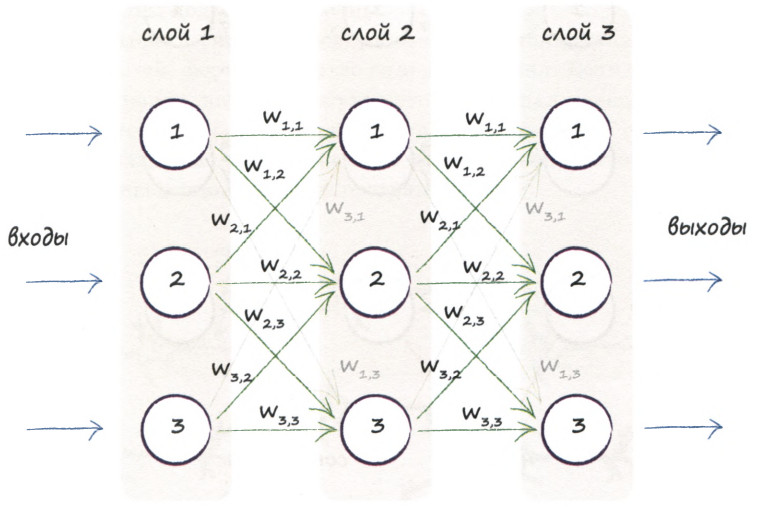
\includegraphics{Parts/images/neural_network.jpg}}
	\caption{Визуализация нейронной сети}
	\label{framework} %framework,fig1
\end{figure}

\indent\setlength{\parindent}{1em} 
Веса синапсов - это одни из параметров нейронной сети и в задачу обучения сети входит подбор весов синапсов так, чтобы минимизировать ошибку модели. Таким образом, подбор весов нейронной сети сводится к задаче минимизации функции ошибки.

\indent\setlength{\parindent}{1em} 
Основной вклад, который внесла статья в развитие распределённого обучения моделей, заключается в том, что авторы разработали два распределенных метода оптимизации и провели серии экспериментов, показывающих эффективность этих моделей по сравнению с нераспределёнными, работающими на CPU или на соптимизированном GPU.

\indent\setlength{\parindent}{1em} 
В статье авторы описывают два распределенных метода оптимизации, которые можно применять для поиска весов нейронной сети: Downpour SGD и Sandblaster L-BFGS. Оба метода были разработаны для фреймворка DistBelief, поддерживающего параллелизм моделей, когда модель делится на части и каждая часть обучается на одном и том же датасете, и параллелизм данных, когда копия модели обучается на разных поднаборах датасета. 

\subsection{Downpour SGD}
\indent\setlength{\parindent}{1em} 
Downpour SGD - асинхронная вариация градиентного спуска SGD. В основе распределенности этой модели лежит параллелизм данных. Несколько копий модели запускаются на разных репликах, каждой реплике отведен поднабор параметров, который она будет менять во время обучения. Модели обмениваются обновленными параметрами с помощью центрального сервера параметров, который хранит текущее состояние всех параметров, которые используются на разных репликах.

\begin{figure}[h]%current location
	\centering
	\scalebox{0.8}{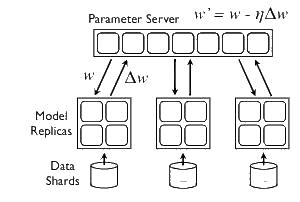
\includegraphics{Parts/images/Downpour_SGD.jpg}}
	\caption{Визуализация Downpour SGD}
	\label{framework} %framework,fig1
\end{figure}

\indent\setlength{\parindent}{1em} 
Преимуществом Downpour SGD по сравнению с синхронной распределенной вариацией SGD является его устойчивость к отказам машин, поскольку каждая реплика индивидуально выполняет свою работу и по завершении не ждет остальных, чтобы обновить значения параметров. Основной проблемой асинхронного подхода является невозможность поддержания консистентности значений параметров для каждой реплики. Поскольку каждая реплика действует независимо, то нет никакой гарантии, что в любой момент времени к параметрам на разных машинах было применено одинаковое количество обновлений или что обновления были применены в одном и том же порядке.

\subsection{Sandblaster L-BFGS}
\indent\setlength{\parindent}{1em} 
Авторы рассматривают распределенное обучение модели L-BFGS, заключающееся в параллелизме данных.  

\indent\setlength{\parindent}{1em} 
Ключевые идеи распределенности для алгоритма L-BFGS, которые предлагают авторы статьи:
\begin{itemize}
  \item распределенное хранение параметров 
  \item выделение процесса координатора, который не имеет доступа к параметрам модели и выступает в роли оркестратора всех реплик, выполняющих обучение
\end{itemize}

\indent\setlength{\parindent}{1em} 
Координатор назначает каждой из реплик модели небольшую часть работы, которую она может выполнить независимо, и каждый раз, когда какая-то реплика заканчивает свою работу, координатор назначает ей новую часть. Такой подход позволяет хорошо использовать быстрые машины и исключает ожидания самой медленной реплики, чтобы продолжить процесс. Результаты работы, а также кэшируемая информация сохраняются локально на каждой реплике и не отсылаются в центральный сервер, что позволяет запускать обучение достаточно больших моделей без оверхеда на отправку и сбор всех параметров. 

\begin{figure}[h]%current location
	\centering
	\scalebox{0.9}{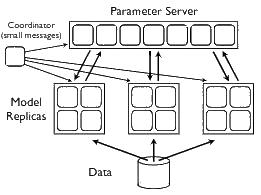
\includegraphics{Parts/images/Sandblaster_L-BFGS.jpg}}
	\caption{Визуализация Sandblaster L-BFGS}
	\label{framework} %framework,fig1
\end{figure}

\subsection{Достигнутые результаты и проверка эффективности}
\indent\setlength{\parindent}{1em} 
Авторы статьи применяют описанные методы оптимизации для двух задач глубинного обучения: распознавание объектов на изображениях и акустическая обработка для распознавания речи.
Ниже приведены графики для задачи обработки речи. Авторы сравнивают три оптимизационных модели, которые тренируются распределённо: Downpour SGD, Downpour SGD w Adagrad, Sandblaster L-BFGS с двумя моделями, которые были обучены на центральном процессоре одной реплики (черная линия) и на оптимизированном графическом процессоре (розовая пунктирная линия).
\begin{figure}[h]%current location
	\centering
	\scalebox{0.9}{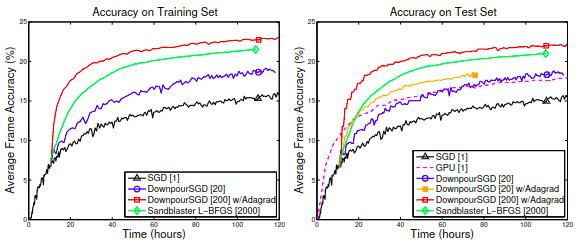
\includegraphics{Parts/images/time_accuracy.jpg}}
	\caption{Зависимость точности модели от времени обучения}
	\label{framework} %framework,fig1
\end{figure}

\indent\setlength{\parindent}{1em} 
Весьма значительным результатом является то, что авторы статьи применили разработанный метод оптимизации к модели с 1.7 миллиардами параметров и получили точность классификации 15\% на кросс валидации, что является относительным улучшением более чем на 60\% по сравнению с лучшей производительностью в этой задаче классификации.


\newpage
%!TEX root = ../main

\newpage
\section{Алгоритм <<All-reduce>>}

Чем больше датасет - тем больше времени тратится на обучение модели по нему. Распределенный синхронный стохастический градиентный спуск - это одно из возможных решений этой проблемы.\cite{DBLP}

\subsection{Описание}
Предположим, у нас есть 8 GPU и мы хотим обучать модель, используя SGD на мини-батчах размера n.

В первую очередь, мы увеличиваем размер батчей до kn, чтобы затем распределить его на k воркеров.
И здесь мы задаемся первым вопросом - а не ухудшится ли точность модели от увеличения размера батча?

Обычно функция потерь для модели имеет следующий вид:
\[L(w) = \frac{1}{|X|} \sum_{x \in X}^{} l(x, w)\]

Здесь $w$ - это параметры модели, $X$ - обучающая выборка, а $l$ -- некоторая функция ошибки,
которая в том числе может включать в себя нормализацию.

Тогда один шаг обучения SGD имеет следующий вид:
\[w_{t + 1} = w_t - \eta \frac1n \sum_{x \in \mathcal{B}}^{} \nabla l(x, w_t)\]

Здесь $\eta$ -- это скорость обучения, гиперпараметр модели, а $\mathcal{B}$ -- текущий батч.

Заметим, что если мы увеличим размер батча в $k$ раз, то количество слагаемых в сумме уменьшится в
$k$ раз. Отсюда вытекает идея: давайте увеличим скорость обучения в $k$ раз, чтобы скомпенсировать
это. И на реальных данных оказывается, что это действительно неплохой подход, который сохраняет
точность модели, за исключением одного случая - начала обучения.

В самом начале, когда модель меняется больше всего, предлагается начать со старой скорости обучения,
равной $\eta$, а затем каждую эпоху увеличивать ее на константу так, чтобы к пятой эпохе она стала
равной $k \eta$. А далее сохраним эту скорость обучения.

Теперь, когда мы научились увеличивать размер батча без особых потерь, будем распределять каждый
батч между воркерами, а затем синхронизировать полученные результаты между ними.

\subsection{Анализ}

Обучалась модель ResNet-50 на датасете ImageNet в течение 90 эпох. В результате модель обучилась за
1 час с размером батча 8192.

Для сравнения, на одной видеокарте с размером батча 256 модель обучается около 29 часов.

При этом самая большая ошибка обучения в датасете увеличилась не более, чем на 0.3\%.



\newpage
%!TEX root = ../main

\newpage
\section{Model parallel \& data parallel}
\indent\setlength{\parindent}{1em} 
Главными подходами для распределенного обучения нейронных сетей является data-parallel и model-parallel. Однако эти подходы не лишены недостатков. В статье "PipeDream: Fast and Efficient Pipeline Parallel DNN Training"\cite{pipedream} описаны основные проблемы данных подходов и предложена система PipeDream, комбинирующая эти методы и тем самым оптимизирующая их.

\subsection{Data parallelism}
Идея Data parallelism заключается в разбиении исходных данных на части, каждая из которых будет использована на отдельной GPU. На каждой GPU находится своя полная копия Нейронной Сети, и веса, получаемые в ходе обучения, синхронизируются между GPU раз в несколько эпох.


\begin{figure}[h]%current location
	\centering
	\scalebox{0.7}{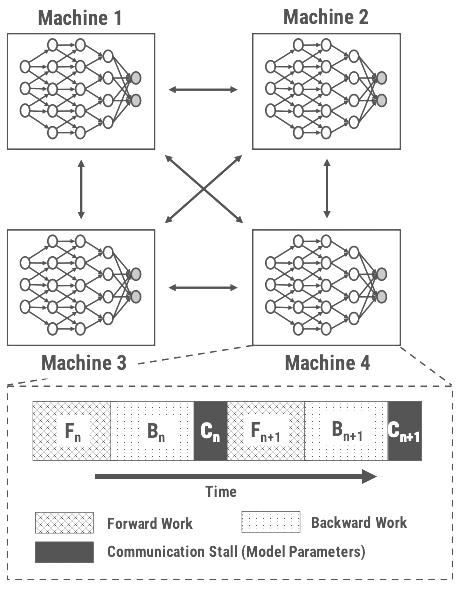
\includegraphics{Parts/images/data-parallel.jpg}}
	\caption{Пример data-parallel на 4 GPU}
	\label{framework} %framework,fig1
\end{figure}

\indent\setlength{\parindent}{1em} 
Однако главная проблема data-parallel заключена в долгом синхронизировании данных между процессами. Были проведены тесты на различных известных нейронных сетях на трех разных видеокартах NVIDIA GPU -- Kepler (K80), Pascal (Titan X) и Volta (V100), и было замерено время, идущее на синхронизацию между процессами:

\begin{figure}[h]%current location
	\centering
	\scalebox{0.7}{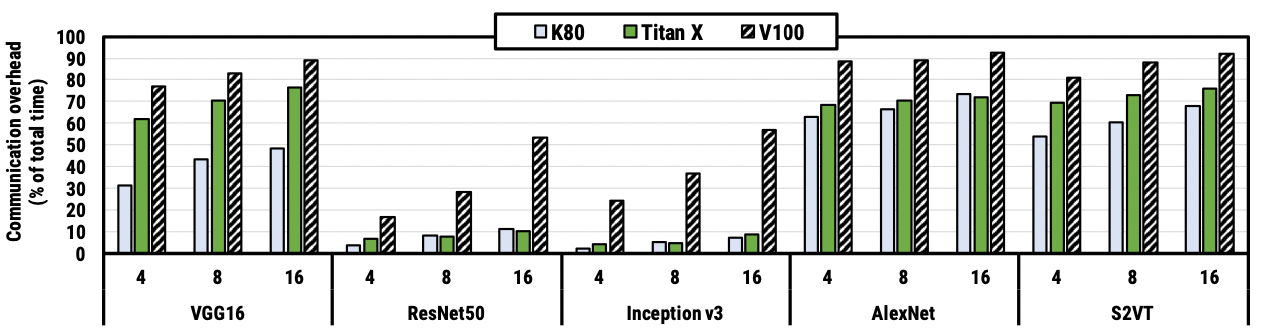
\includegraphics{Parts/images/communication-overhead.jpg}}
	\caption{Время на синхронизацию в \% от всего времени обучения DNN}
	\label{framework} %framework,fig1
\end{figure}

\indent\setlength{\parindent}{1em} 
Как видно на данном графике, время, занимаемое на синхронизацию , может достигать до 90\% от всего времени обучения DNN.

\newpage
\subsection{Model Parallelism}
Идея Model Parallelism заключается в разбиении самой модели на несколько частей, каждая из которых будет вычисляться на отдельной GPU. Данный подход часто используется в Машинном Обучении (ML). Однако для DNN наивный подход model-parallel имеет огромный недостаток. Разбивая Нейронную Сети на части по несколько слоев Нейронной Сети, отдельная часть должна вычисляться только после вычисления предыдущей части:

\begin{figure}[h]%current location
	\centering
	\scalebox{1}{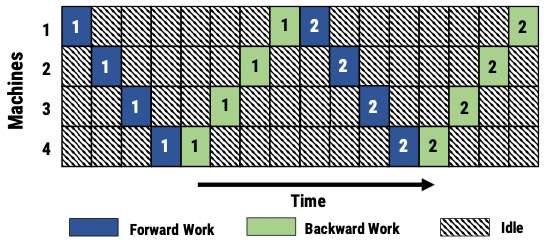
\includegraphics{Parts/images/model-parallel.jpg}}
	\caption{Процесс наивного model-parallel на 4 GPU. \\Числа обозначают номер батча.}
	\label{framework} %framework,fig1
\end{figure}

\indent\setlength{\parindent}{1em} 
Из-за такого подхода наши GPU значительную часть времени находятся в режиме ожидания, и как такового прироста в производительности нет.

\subsection{PipeDream}
\indent\setlength{\parindent}{1em}  
PipeDream использует идею model-parallel, деля DNN на части по несколько слоев Нейронной Сети, но при этом, прямые и обратные проходы для разных батчей будут выполянться параллельно, тем самым минимизируя работу GPU в режиме ожидания.

\begin{figure}[h]%current location
	\centering
	\scalebox{1}{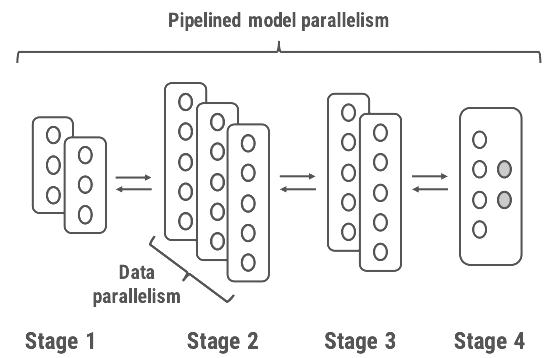
\includegraphics{Parts/images/pipelined_model_example.jpg}}
	\caption{Процесс обучения PipeDream, объединяющий data-parallel и model-parallel}
	\label{framework} %framework,fig1
\end{figure}

\newpage
\subsubsection{Распределение слоев между GPU}
\indent\setlength{\parindent}{1em}  
Для минимизации времени работу GPU в режиме ожидания важно правильно поделить DNN на части. Главная задача при разделении заключается в том, что каждая отдельная компонента PipeDream выполнялась одинаковое количество времени.

Для этого вначале производится замер времени работы DNN, производя вычисления 1000 батчей на одной из GPU. После этого при помощи динамического программирования находится оптимальное разделения на части, каждая из который будет вычисляться одинаковое количество времени (тогда мы можем считать, что каждая часть выполняется ровно одну единицу времени).

\begin{figure}[h]%current location
	\centering
	\scalebox{0.7}{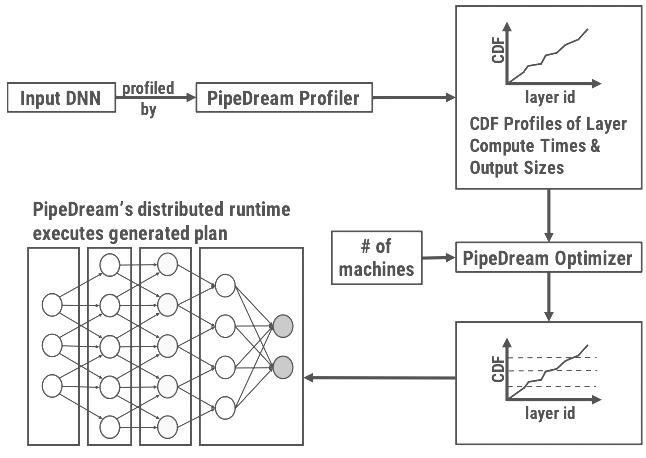
\includegraphics{Parts/images/pipedream_process.jpg}}
	\caption{Автоматизированный процесс деления DNN на части}
	\label{framework} %framework,fig1
\end{figure}

\subsubsection{Последовательность вычисления}
\indent\setlength{\parindent}{1em}
В отличие от обычных реализаций pipeline, в которых одновременно вычисления происходят только либо в прямом, либо в обратном порядке, в PipeDream вычисления происходят в обе стороны одновременно. То есть у каждой GPU в каждую единицу времени есть выбор: либо делать прямой проход графа вычислений, либо обратный. 

\begin{figure}[h]%current location
	\centering
	\scalebox{0.7}{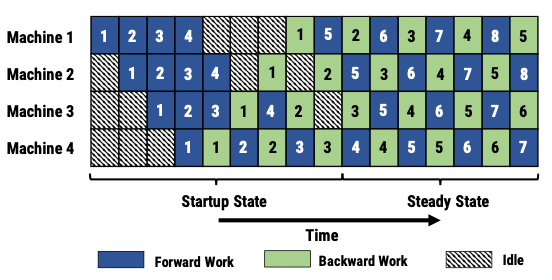
\includegraphics{Parts/images/pipedream_work_schedule.jpg}}
	\caption{Автоматизированный процесс деления DNN на части}
	\label{framework} %framework,fig1
\end{figure}

\indent\setlength{\parindent}{1em}  
В начальной стадии использнения PipeDream, первая часть получает на вход оптимальное количество батчей, последовательно после вычисления передавая следующей части (а значит и следующей GPU) результат вычисления. 

\indent\setlength{\parindent}{1em}  
В основной стадии работы PipeDream на одной GPU чередуются прямой и обратный проходы. Такой механизм авторы статьи назвали one-forward-one-backward (1F1B).

\newpage
\subsubsection{Эффективность обучения}
\indent\setlength{\parindent}{1em} 
Как мы можем видеть из примера из последней иллюстрации: прямой проход для батча №5 для первой GPU проходит после обновления весов после обратного прохода батча №1. При этом обратный проход батча №5 проходит после оборатных проходов батчей №2, №3 и №4. Это может негативно влиять на сходимость.

\indent\setlength{\parindent}{1em}
\textbf{Weight Stashing:} в PipeDream реализована идея сохранения весов для всех батчей, которые в данный момент времени вычисляются в модели. Таким образом, когда батчу нужно пройти прямой проход, то используются последняя версия весов. После этого сохраняется версия весов, которая вспоследствии будет использована при обратном проходе того же батча. Такой метод авторы статьи называют Weight Stashing. Благодаря ему для каждой части модели для каждого батча используются подходящие веса, как для прямого, так и для обратного проходов. Тем самым не будет нарушена сходимость графа вычислений.

\subsection{Заключение}
\indent\setlength{\parindent}{1em} 
PipeDream существенно превосходит метод data-parallel, посколько каждая GPU обменивается только частью параменторв (таким образом синхронизация происходит быстрее):

\begin{figure}[h]%current location
	\centering
	\scalebox{0.7}{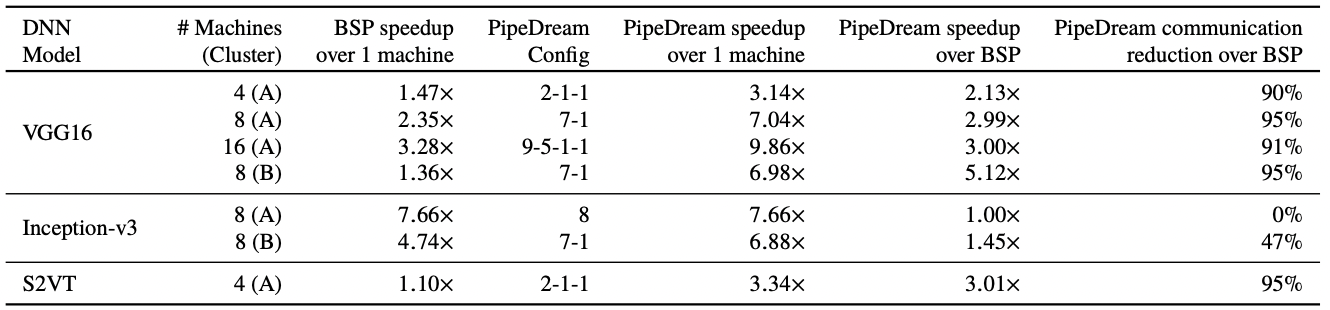
\includegraphics{Parts/images/pipedream_tests.jpg}}
	\caption{Сравнение PipeDream с data-parallelism (BSP)}
	\label{framework} %framework,fig1
\end{figure}

\indent\setlength{\parindent}{1em} 
По резуьтатам экспериментов для моделей VGG16 и S2VT время, затраченное на синхронизацию, уменьшилось на 90\%, при этом в целом модель стала в среднем обучаться в 3 раза быстрее.

\newpage
%!TEX root = ../main

\section{Tensor Parallelism NLP}

Рассмотрим, что нам предлагают авторы статьи <<Megatron-lm: Training multi-billion parameter language models using model parallelism>>\cite{shoeybi2019megatron}.

\subsection{Многопоточное обучение}

У нас есть классные задачки на NLP, модели GPT-2 и Bert, которые достигли State-of-the-art (выдающихся результатов) в решении каких-то сложных задач. Но есть проблема - они состоят из большого количества параметров и требуют довольно много данных чтобы обучится. В итоге обучить их становится довольно трудно, если использовать только один процессор.

\begin{wrapfigure}[30]{r}{0.55\textwidth}
    %\vspace{-2cm}
	\begin{center}
        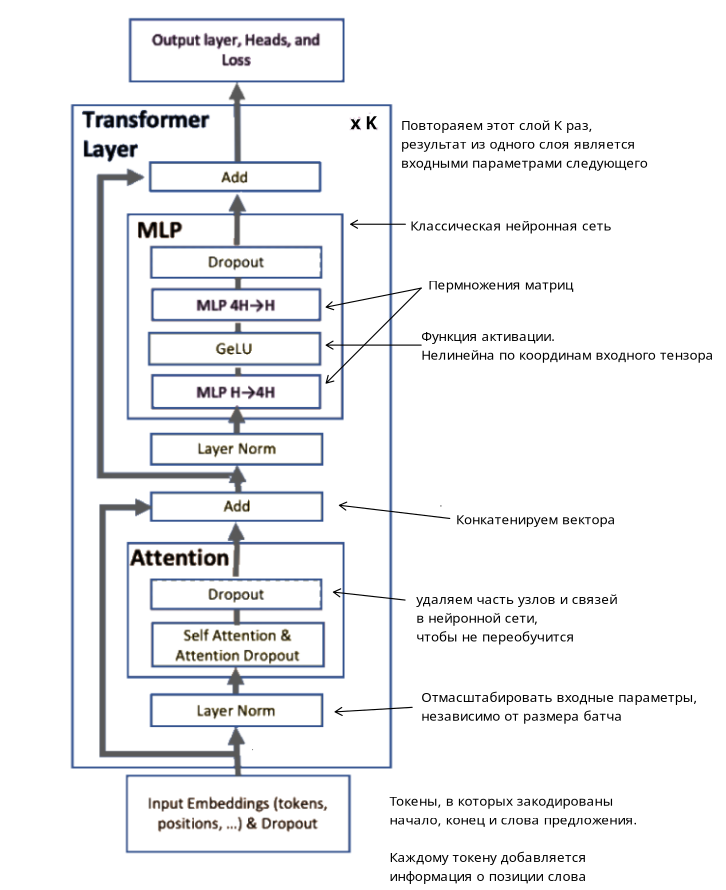
\includegraphics[width=1.2\linewidth]{Parts/images/TP_Transformer.png}
	\end{center}
	\caption{модель трансформера, взятая авторами статьи}
    \label{fig:transformer1}
\end{wrapfigure}

Поэтому люди делают обучение многопоточным. Некоторые популярные способы: 
\begin{enumerate}
    \item Разбивают данные на партии (batch-и), и их отдают модели параллельно на несколько GPU. Затем результаты агрегируются через функцию (например берется среднее градиентов для последующего изменения весов модели)
    \item  Делают модель распределенной. Разбивают модель на набор операций, и разносят их по процессам, а затем синхронизируют. Здесь нужна дополнительная логика поверх используемой модели. 
\end{enumerate}


\subsection{Авторский подход}
Авторы используют немного другой подход. Одни из самых частых операций - это вычисления с тензорами (например перемножения матриц). Поэтому можно разбить тензор параметров модели на несколько, все полученные составляющие раскидать по разным GPU, каждому отдать одни и те же входные данные, и запустить параллельную обработку. Если в модели есть нелинейный слой, требующий всех данных сразу - собрать результат с всех процессоров и пропустить через нее. Чем меньше точек синхронизации, тем лучше производительность. А из-за того, что мы разбиваем элементы модели, не меняя особо процесс ее обучения - то изменения нужны минимальные.


Описанные дальше подходы можно применять для любой подходящей модели, но авторы взяли задачи NLP. В основе наиболее успешных моделей лежат трансформеры (Transformers). Его истоки состояли из RNN - что вообще не ложится на параллельность. Но \cite{vaswani2017attention} от реккурентости избавляются, что позволяет обрабатывать входные данные и выполнять некоторые слои параллельно. Теперь трансформеры - корень всех моделей, их можно разбить на encoder-а и decoder-а, собирать их последовательно, навешивать дополнительные слои, обучать модели для разных задач и получать удивительные результаты. Bert обучался понимать структуру языка, изначально решая набор базовых задач (как вставить правильное слово в пропуск и сказать про предложения - они связаны или нет). Затем он дообучается для более конкретной задачи. GPT-2 это модель которая умеет по началу предложения генерировать продолжение. Сначала GPT уступало Bert, но разработчики значительно увеличили количество параметров до 1.5 млдр, сделав ее самой большой на тот момент, разнообразили датасет из статей из интернета, и она достигла воистину state-of-the-art, ее даже боялись публиковать полностью. Поэтому чтобы ускорить модели, можно оптимизировать именно трансформеры.

Модель трансформера, взятая авторами статьи: \ref{fig:transformer1}

% \begin{wrapfigure}[12]{r}{0.55\textwidth}
%     \vspace{-1cm}
% 	\begin{center}
%         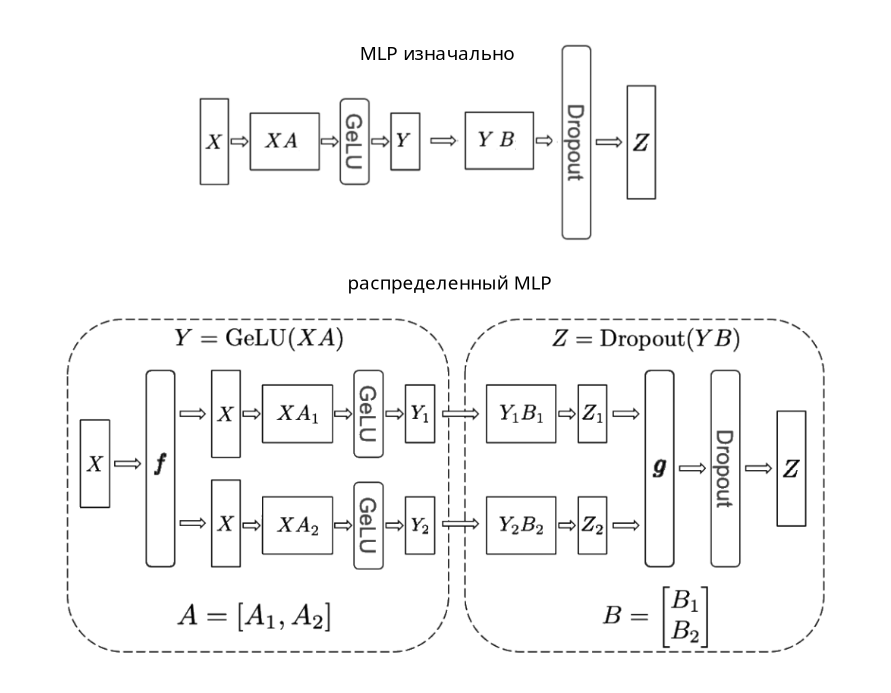
\includegraphics[width=0.95\linewidth]{Parts/images/TP_MLP.png}
% 	\end{center}
% 	\caption{Преобразования MLP}
%     \label{fig:transform2}
% \end{wrapfigure}

Найдем, где в этой модели используется перемножение матриц. В более простом блоке нашей модели - MLP преобразования будут следующими:

\begin{figure}[H]
    \centering
    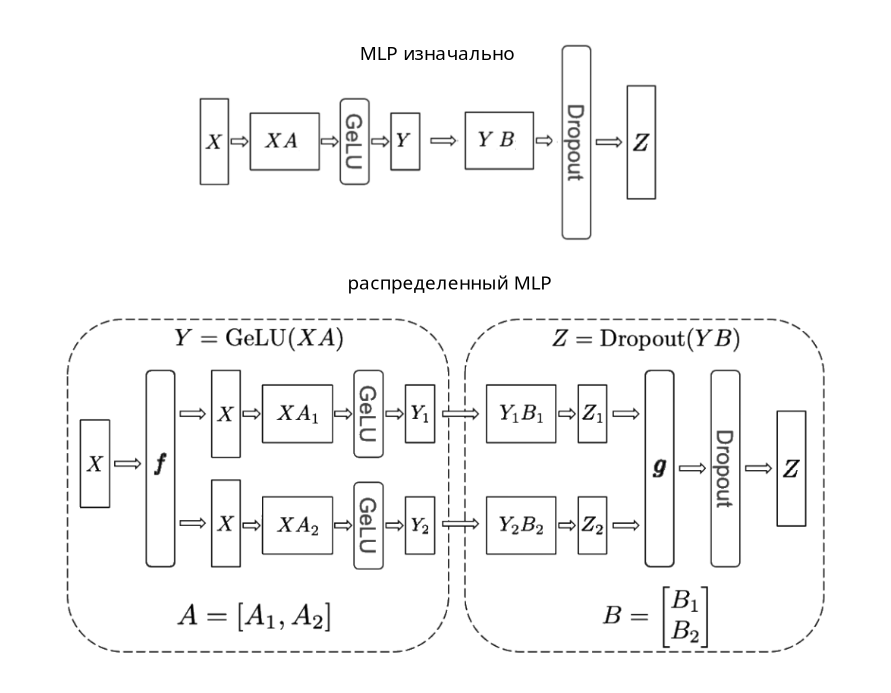
\includegraphics[width=0.8\linewidth]{Parts/images/TP_MLP.png}
    \caption{Преобразования MLP}
\end{figure}

Если посмотреть на них внимательно, то обе схемы почти одинаковые. Только в нижней есть блок f, который в прямом проходе дублирует данные на несколько GPU, и блок g - который собирает данные с нескольких процессоров в одну матрицу. Эти блоки являются точками синхронизации, и их на каждый проход (прямой и обратный для релаксации весов) по 2 для одного Transformer Layer-а. 


Аналогично поступаем и для слоя внимания:

\begin{figure}[H]
    \centering
    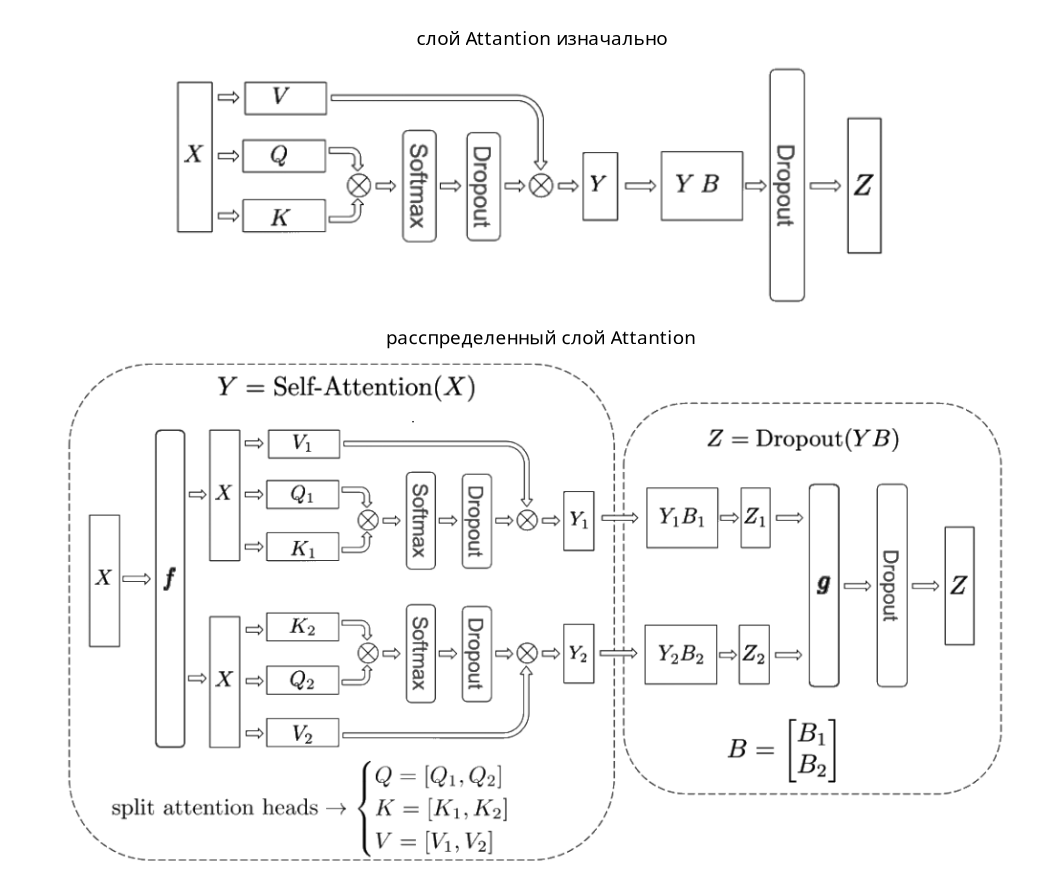
\includegraphics[width=0.8\linewidth]{Parts/images/TP_Attention.png}
    \caption{Преобразования Attention}
\end{figure}


% \begin{figure}
%     \hspace{-1cm}
%     \centering
%     \begin{subfigure}[b]{0.5\textwidth}
%         \centering
%         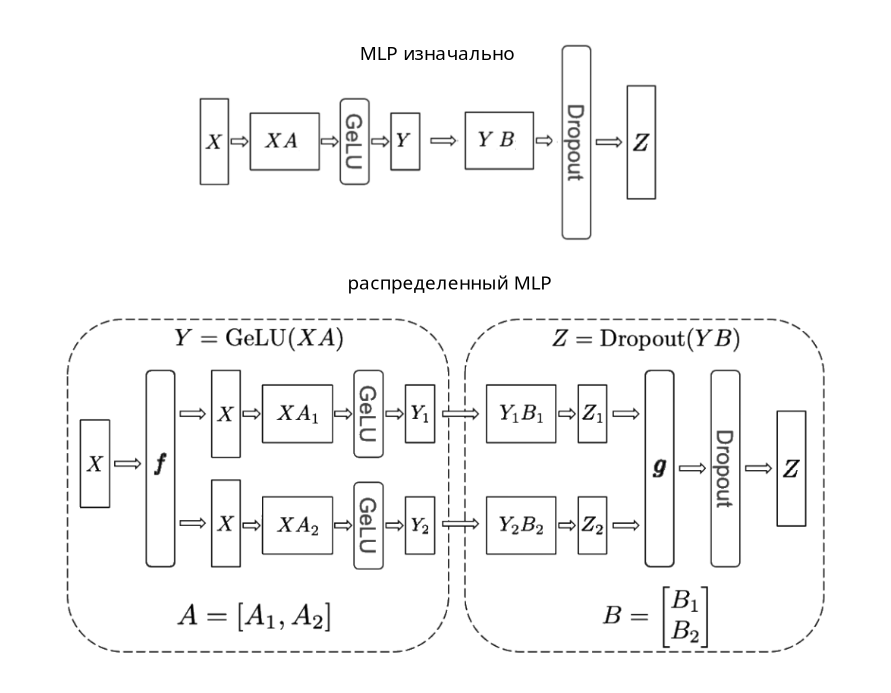
\includegraphics[width=0.95\linewidth]{Parts/images/TP_MLP.png}
%         \caption{MLP}
%     \end{subfigure}
%     \begin{subfigure}[b]{0.5\textwidth}
%         \centering
%         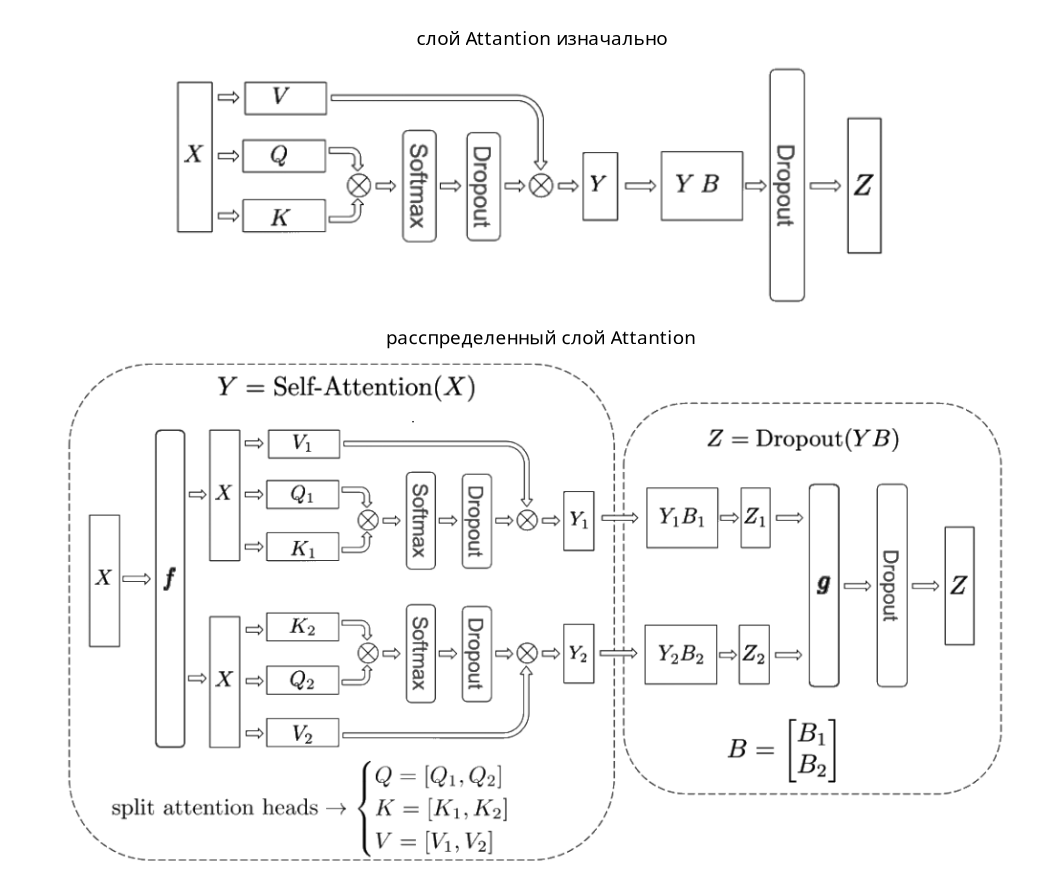
\includegraphics[width=0.95\linewidth]{Parts/images/TP_Attention.png}
%         \caption{Attention}
%     \end{subfigure}
%     \caption{Преобразования}
% \end{figure}

Получаем распараллеленную модель, добавив всего два простых блока f и g.


Некоторые модели могут отличаться от представленного в статье, но почти любое перемножение матрица можно параллелить, не забывая потом добавлять простой объединяющий слой когда нужно. 

Еще одно  улучшение - перед тем, как считать cross entropy, мы должны отправить одному процессору объединенную матрицу. Одной из ее размерностью является размер словаря, что для хороших моделей будет большой. Там будут находится вероятности для данного слова быть в предложении следующим. Так вот, всю эту размерность можно схлопнуть, если считать  cross entropy на каждом GPU работающем параллельно, и отправлять уже меньше данных. Авторы говорят, что это сильно улучшило их время обучения. 

Теперь интересно посмотреть на то, как хорошо это работает.

Для обучения моделей был собран единый датасет из существующих (тексты с Википедии, новостей и тд), который весил 174 Гибибайт. 

Сначала применили паралелизацию описанную выше для 1-2-48 GPU, и посмотрели на эффективность (на графике синие столбца). Раньше я также говорила про один из способов ускорить обучение - разбить данные на batch-и. Это называется data parallel, и его можно также внедрить в схему. До этого мы обучающие данные копировали полностью на несколько GPU, и на каждом работали с разными весами модели. Теперь можно вместо одной GPU в схеме, поставить 64 идентичных, полностью скопировать внутреннее состояние, а вот входные данные разбить между ними. Получается что так мы сначала делим модель, а затем входные embedding-и. Используемых GPU получаем больше, измеряем эффективность распределенных вычислений на них и рисуем зеленные столбцы.

\begin{figure}[H]
    \centering
    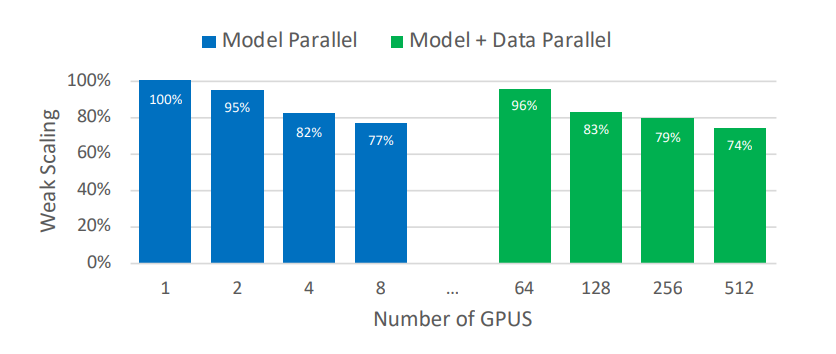
\includegraphics[width=0.8\linewidth]{Parts/images/TP_weak_scaling.png}
    \caption{Эффективность распределенных вычислений}
\end{figure}


Что вообще на этом графике изображено и про что weak scaling? Для его измерения мы увеличиваем количество GPU и количество входных данных нашего датасета для нашей модели. В идеальном мире, время работы каждого отдельного процессора не должно изменится, ведь он обрабатывает одно и тоже количество данных, и это мы называем 100\%. Но в реальном мире у нас есть накладки например в виде времени обмена данными между GPU, и поэтому время работы немного увеличивает по сравнению с идеальным вариантом. Weak Scaling здесь показывает эффективность наших действий с добавлением большего числа GPU по сравнению с идеальным вариантом.

В итоге, авторы статьи достигают 77\% и 74\% по сравнению с наилучшим вариантом, в котором бы при увеличении размера входных данных время обучения бы не изменилось. Чтобы как-то ощутить сколько это хорошо, модель GPT-2 которая имеет 355 миллиона параметров обучалась одну эпоху за 20.6 часов, а модель с 8.3 миллиардами (в 23 раза больше) - за 50.4 часов, что является самой большой моделью, что когда-либо собирали на момент написания статьи.

Более того, большие модели показывают лучше результат - на графиках видно, что чем больше параметров у модели, тем меньше функции потерь. На втором графике архитектура (a) (классический Bert) от архитектуры (b) (на что мы смотрели в этой статье) отличается количеством вектором, проходящих через слов Layer Norm. Как видно на графике, у классического Bert-а с большим числом параметров начинает переобучение, поэтому авторам статьи пришлось изменить модель.  


\begin{figure}[H]
    \centering
    \scalebox{1.1}{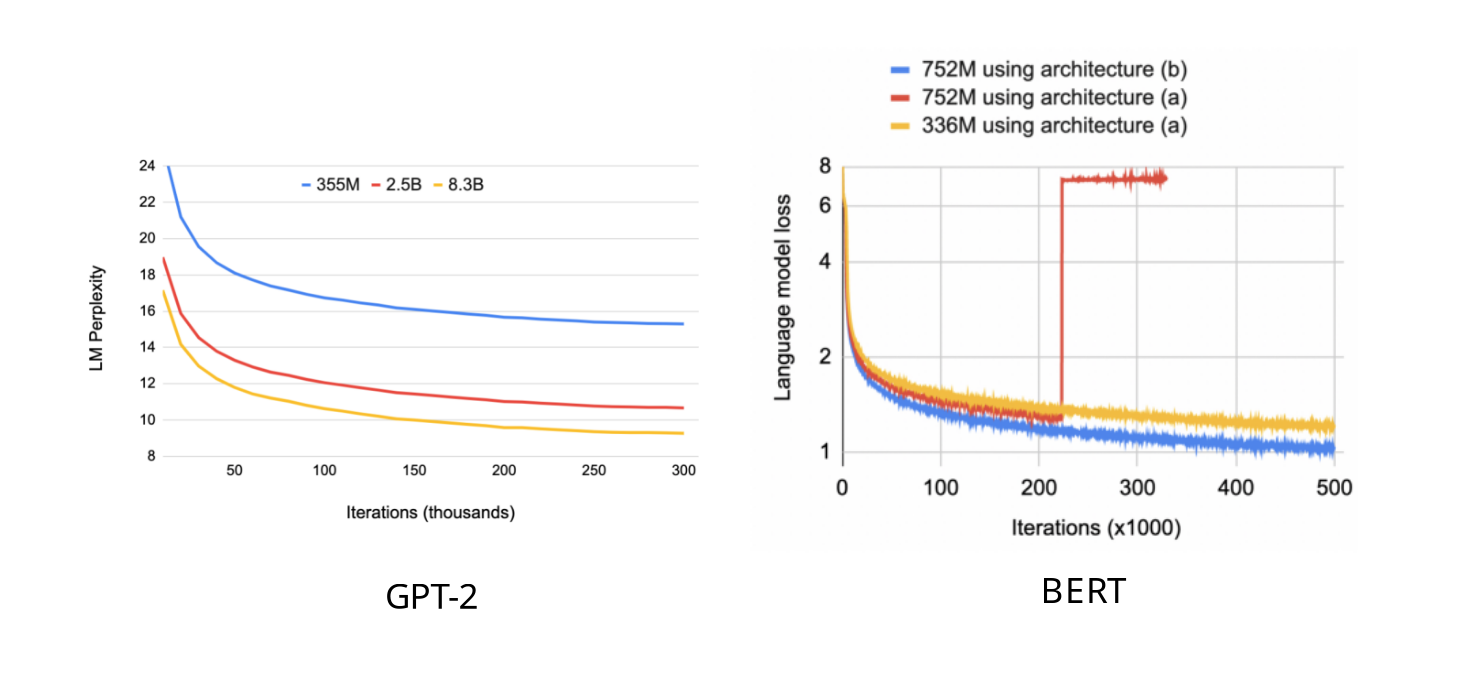
\includegraphics[width=\linewidth]{Parts/images/TP_loss.png}}
    \caption{Сравнение моделей Bert и CPT-2}
\end{figure}


\subsection{Заключение}

Суммируя рассказ, модели нейронных сетей с большим количеством параметров могут работать лучше, но также требуют значительно больше временных ресурсов чтобы обучится. Можно использовать больше процессоров, и внеся довольно мало изменений в работу программ, в итоге получить результаты за более разумное время.


\newpage
\addcontentsline{toc}{section}{Список литературы}
\printbibliography

\addcontentsline{toc}{section}{Список иллюстраций}
\listoffigures

%\newpage 
%%!TEX root = ../main

\section{Распределение обязанностей в команде}

\begin{itemize}
    \item Иван Ершов -- анализ статьи \cite{pipedream}
    \item Дарья Жукова -- анализ статьи \cite{beginning}
    \item Ксения Петренко -- анализ статьи \cite{shoeybi2019megatron} и \cite{vaswani2017attention}
    \item Тагир Хамитов -- анализ статьи \cite{DBLP}
    \item Артём Макогон -- сборка, оформление \href{https://github.com/makogon2907/HSE-Practice-Fall-2022}{отчета}
    \item Дмитрий Брусенин -- сборка, оформление \href{https://github.com/makogon2907/HSE-Practice-Fall-2022}{отчета}
\end{itemize}


\end{document}
% Начиная с этого момента весь текст LaTeX игнорирует, можете вставлять любую абракадабру.
